\label{task4}
% 4. Describe an architecture for the control system (preferably using pictures).
\section{Architecture}
The architecture for the control system is designed with the set of controllers mentioned in the problem statement. The control systems are segregated into input controller, sensory controller and output controller. 
\subsection{Console Input Controller}
Input controller consists of the console inputs to MPSP which are Up, Down, Stop, Resume, Undock and Reset. Since the action requirements can be set according to preference, we are assuming a simplistic approach of button press and release. The button can be continuously pressed for a respective continuous action and then released.

\begin{figure}[htp]
    \centering
    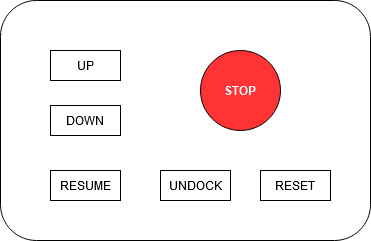
\includegraphics[width=4cm]{chapters/images/Console.png}
    \caption{Input Controller}
    \label{fig:inputController}
\end{figure}

\subsection{Sensor Input Controller}
Sensor controller consists of sensors to identify the location of the bed and docking activity of the MPSP unit. This controller senses the horizontal location, vertical location and docking status (docked or undocked).  Furthermore, it also senses the calibrated standard height, uncalibrated maximum height, uncalibrated minimum height, horizontal leftmost position, horizontal rightmost position. To further simplify the model, it is assumed that this controller senses the manual motion in the case of an emergency situation as well.

\subsection{Output Controller}
The third controller is the output controller, which activates the responses for the input controller based on certain requirement logics. This controller hence controls the motors and brakes including the docking and undocking mechanism. The overall  systems included in this are horizontal motor, horizontal brake, vertical motor, vertical brake and docking spring.

\begin{figure}[htp]
    \centering
    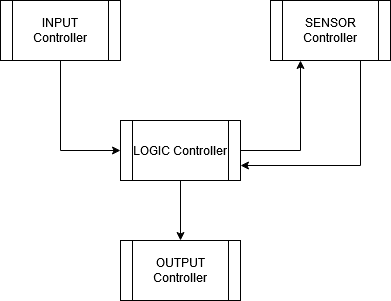
\includegraphics[width=4cm]{chapters/images/Architecture.png}
    \caption{Architecture Overview}
    \label{fig:architecture}
\end{figure}

To simplify and add the requirement logics to the input-output actions, a further logic controller is added which receives live inputs from the input controller and sensory controller and based on the input requirements the corresponding action is sent to the output controller. It also helps in keeping track of the previous state and current state. This helps in case of recovering from an emergency stop action if the current state is invalid to bring it back to a correct state.

So whenever an input action is initiated, the logic controller gets input from the input controller as well as gets live sensory info from the sensory controller and based on the requirements logic provides the suitable action that is sent to the output controller. All the channels are assumed to have zero latency. The channel is unidirectional from input to logic, bidirectional from logic to sensory and unidirectional from logic to output controllers.
